\newpage
\section{Thiết kế giao diện}

\subsection{Giao diện đăng nhập}
Trang hiển thị giao diện khi người dùng (người quản lý trang trại, người quản lý) đăng nhập
vào hệ thống bằng cách nhập thông tin tài khoản và mật khẩu
\begin{figure}[H]
  \centering
  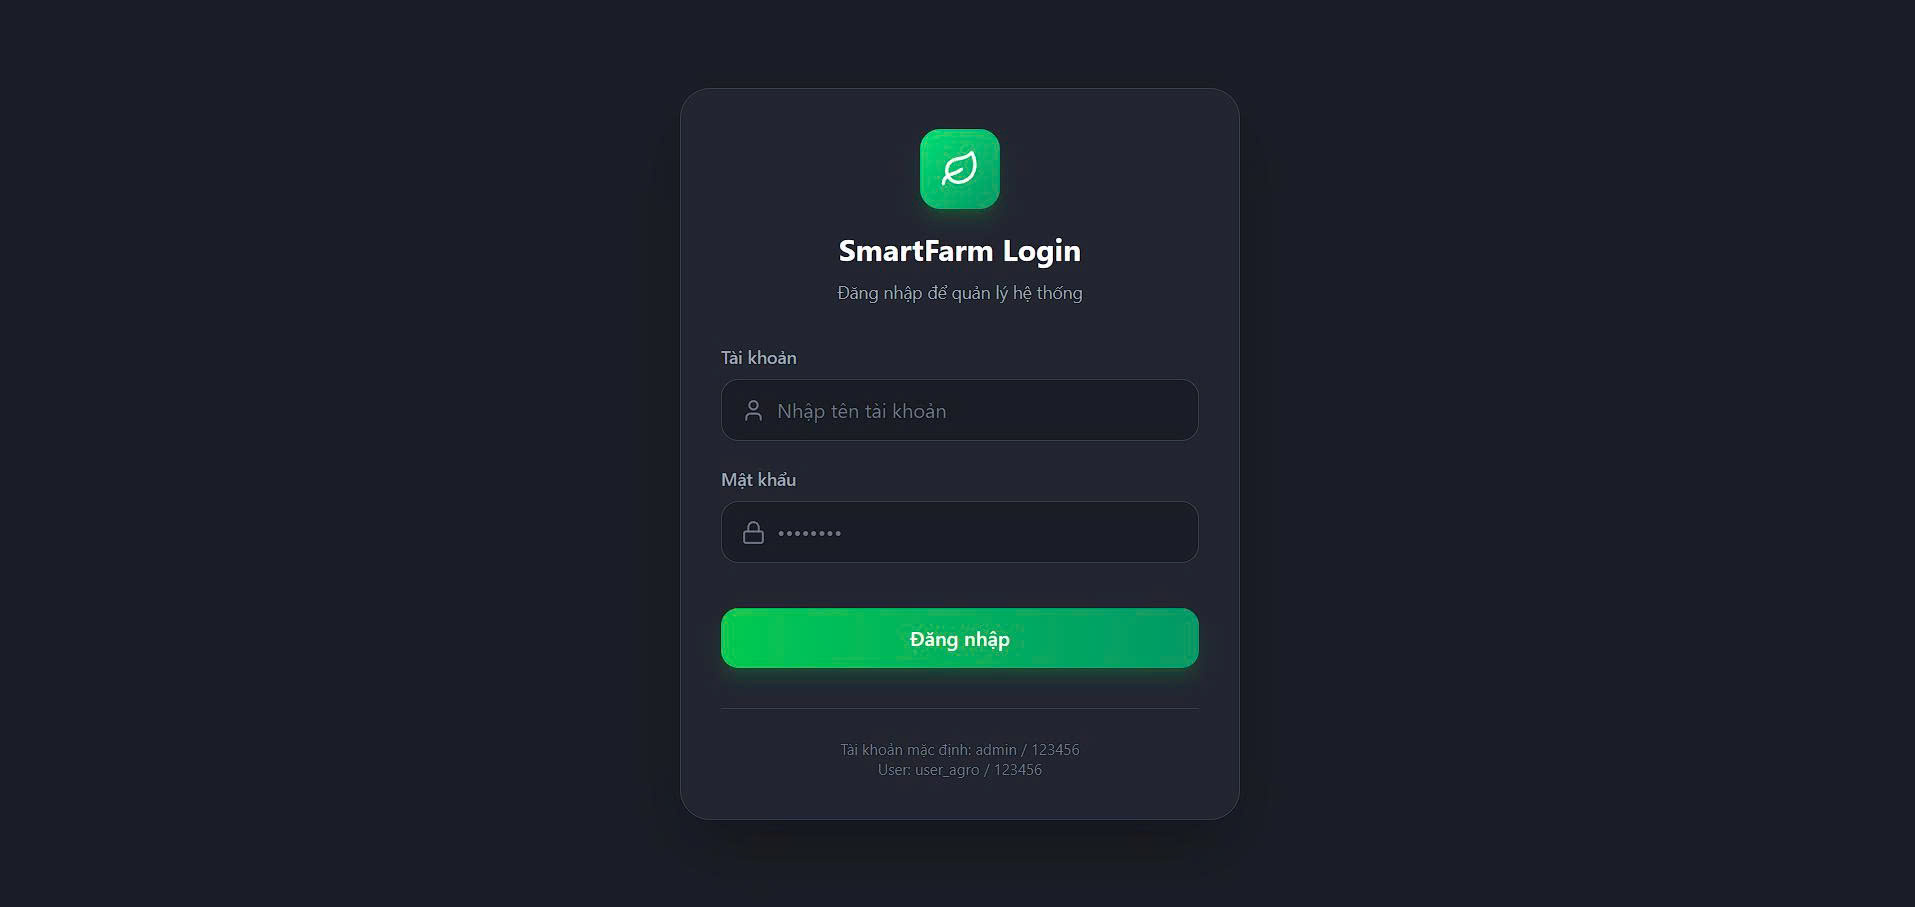
\includegraphics[width=0.8\textwidth]{img/dangnhap.jpg}
  \caption{Giao diện đăng nhập chính của hệ thống quản lý nông trại thông minh}
  \label{fig:interface}
\end{figure}

\subsection{Giao diện quản lý nông trại}
Sau khi đăng nhập thành công, màn hình sẽ xuất hiện giao diện hiển thị các khu vườn mà
người dùng đang quản lý.
\begin{figure}[H]
  \centering
  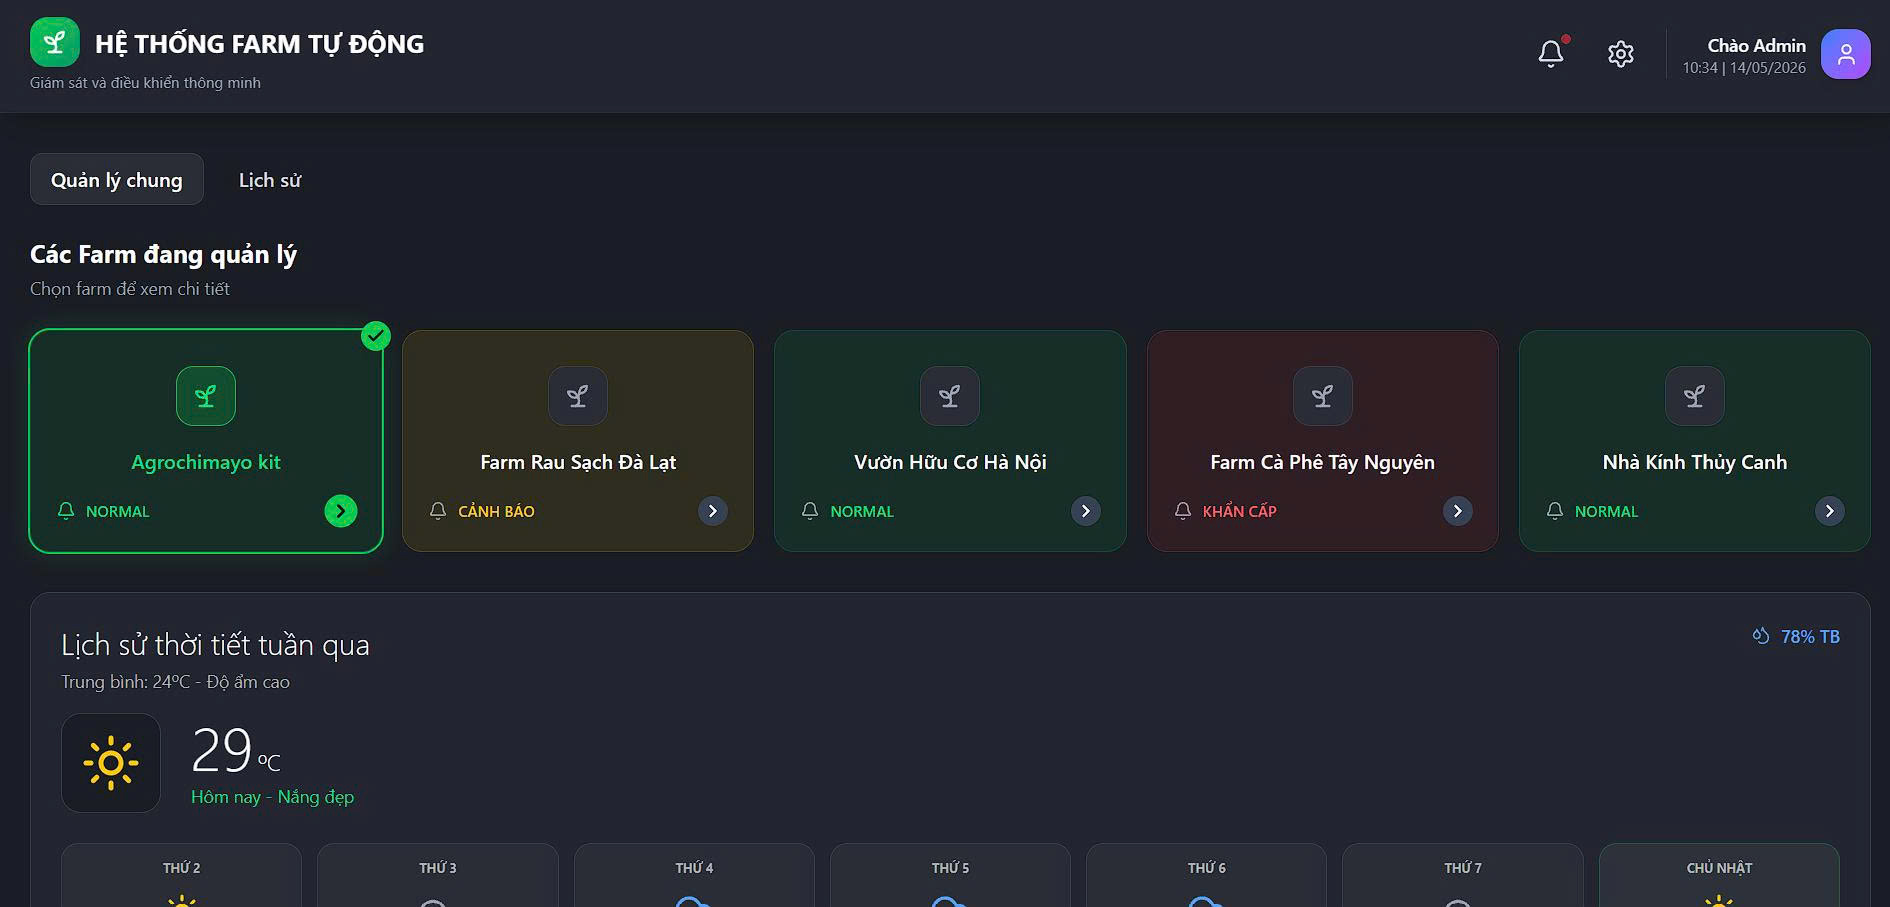
\includegraphics[width=0.8\textwidth]{img/chonfarm.jpg}
  \caption{Giao diện chọn nông trại}
  \label{fig:interface}
\end{figure}
\subsection{Giao diện xem dữ liệu Realtime}
Khi chọn vào khu vườn bất kỳ thì sẽ hiển thị các thông số về: nhiệt độ, độ ẩm đất, độ ẩm
không khí, cường độ ánh sáng ở thời điểm hiện tại và các thông tin về thời tiết trong các ngày gần đây
\begin{figure}[H]   
  \centering
  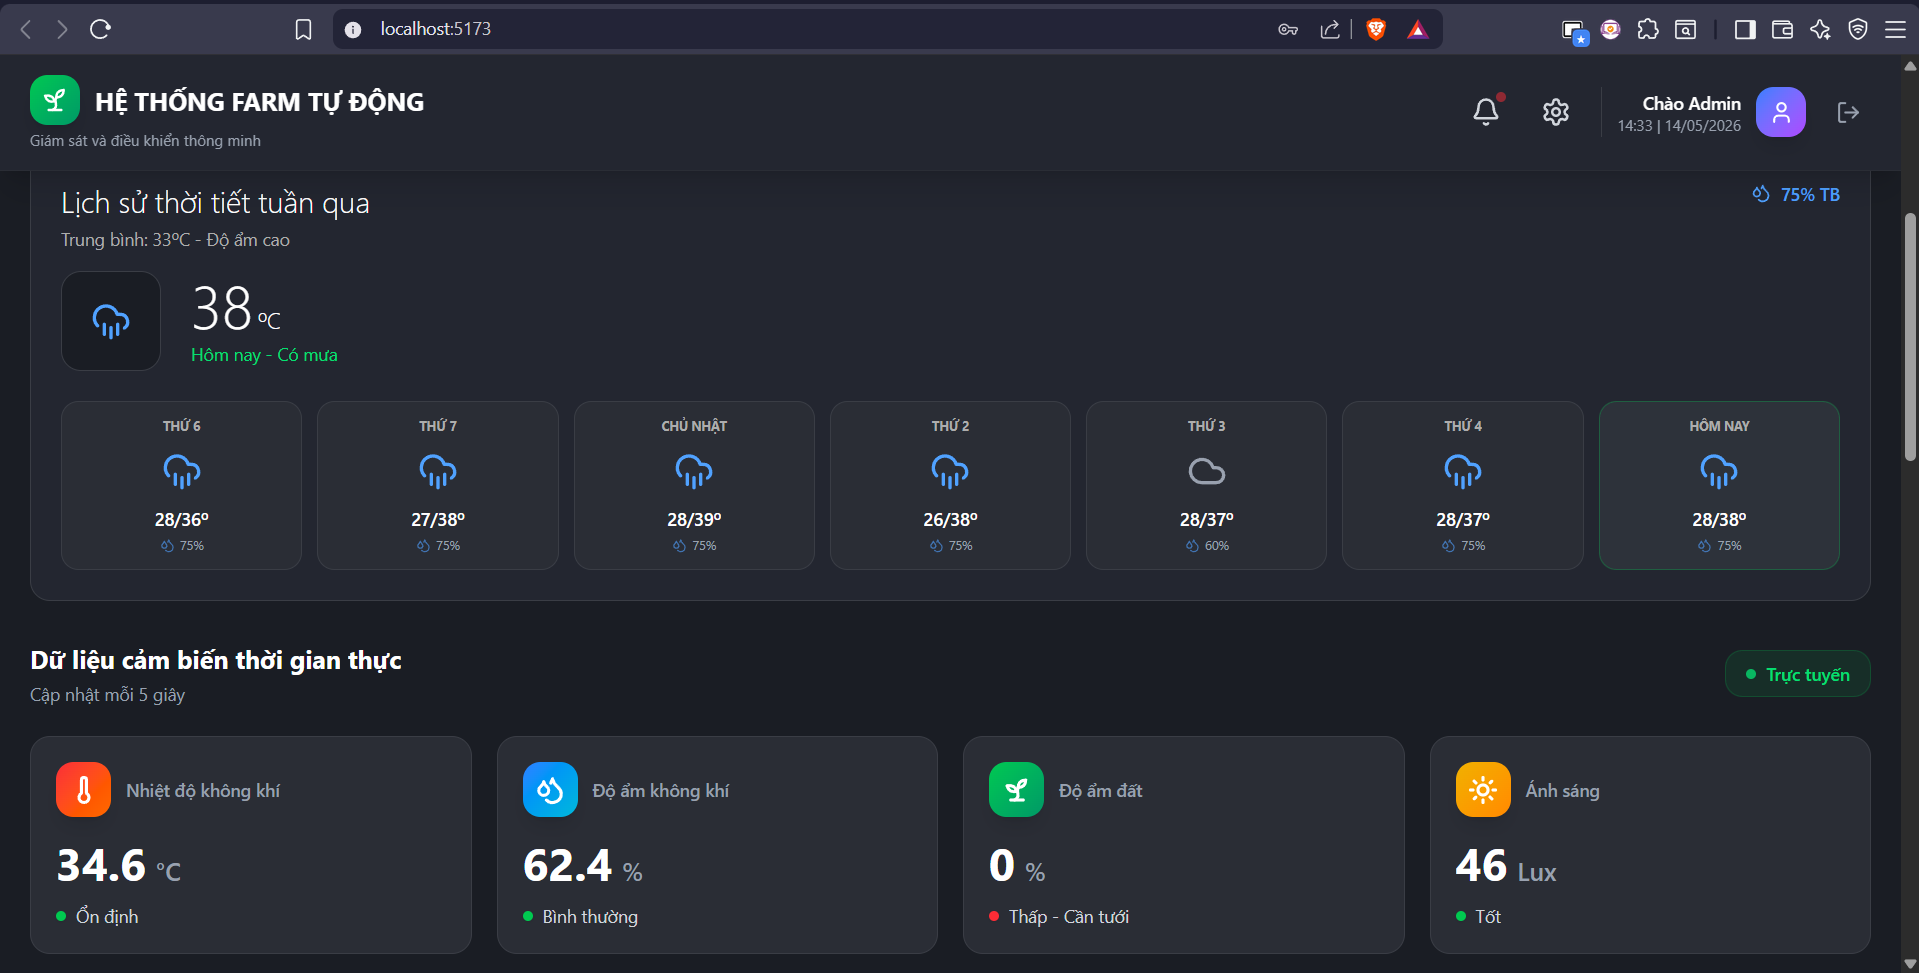
\includegraphics[width=0.8\textwidth]{img/xemdulieu.png}
  \caption{Giao diện xem dữ liệu Realtime}
  \label{fig:interface}
\end{figure}

\subsection{Giao diện điều khiển thiết bị}
\subsubsection{Điều khiển máy bơm}
\begin{figure}[H]
  \centering
  % Hình bên trái
  \begin{subfigure}[b]{0.49\textwidth}
    \centering
    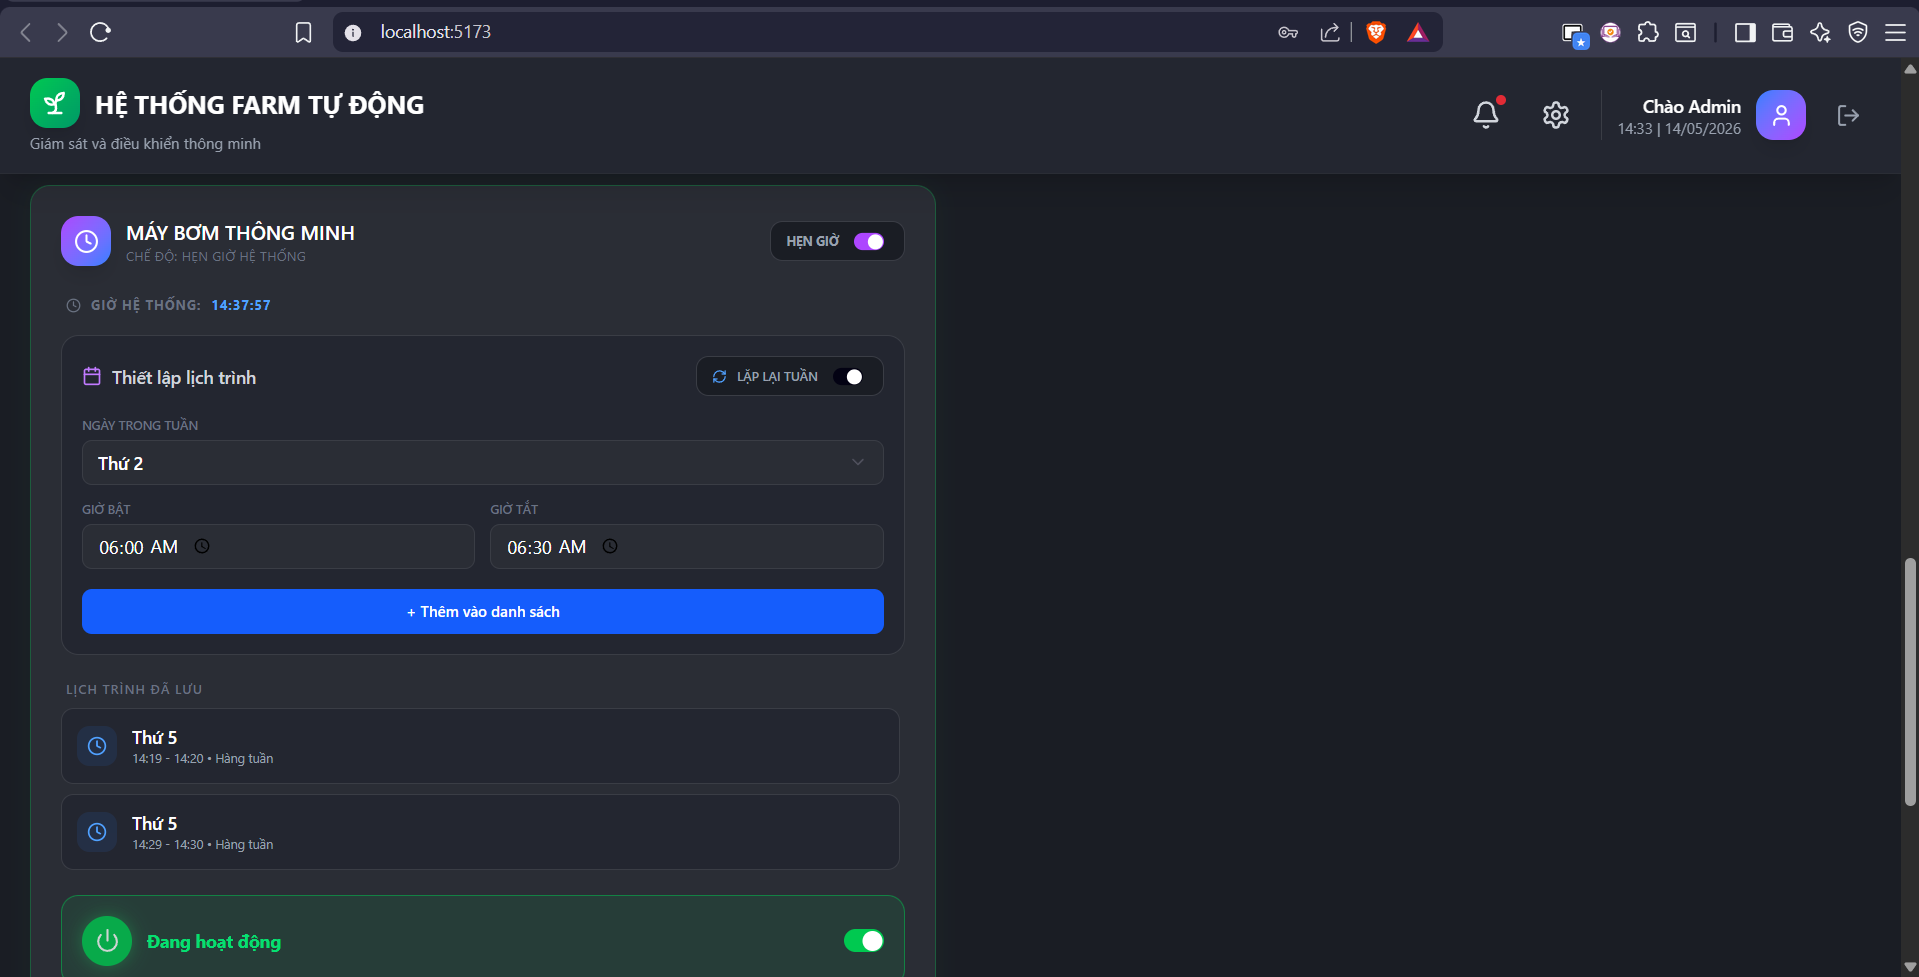
\includegraphics[width=\textwidth]{img/maybomtheogio.png}
    \caption{Giao diện điều khiển máy bơm theo thời gian hẹn trước}
    \label{fig:interface1}
  \end{subfigure}
  \hfill % Tạo khoảng trống ở giữa hai hình
  % Hình bên phải
  \begin{subfigure}[b]{0.49\textwidth}
    \centering
    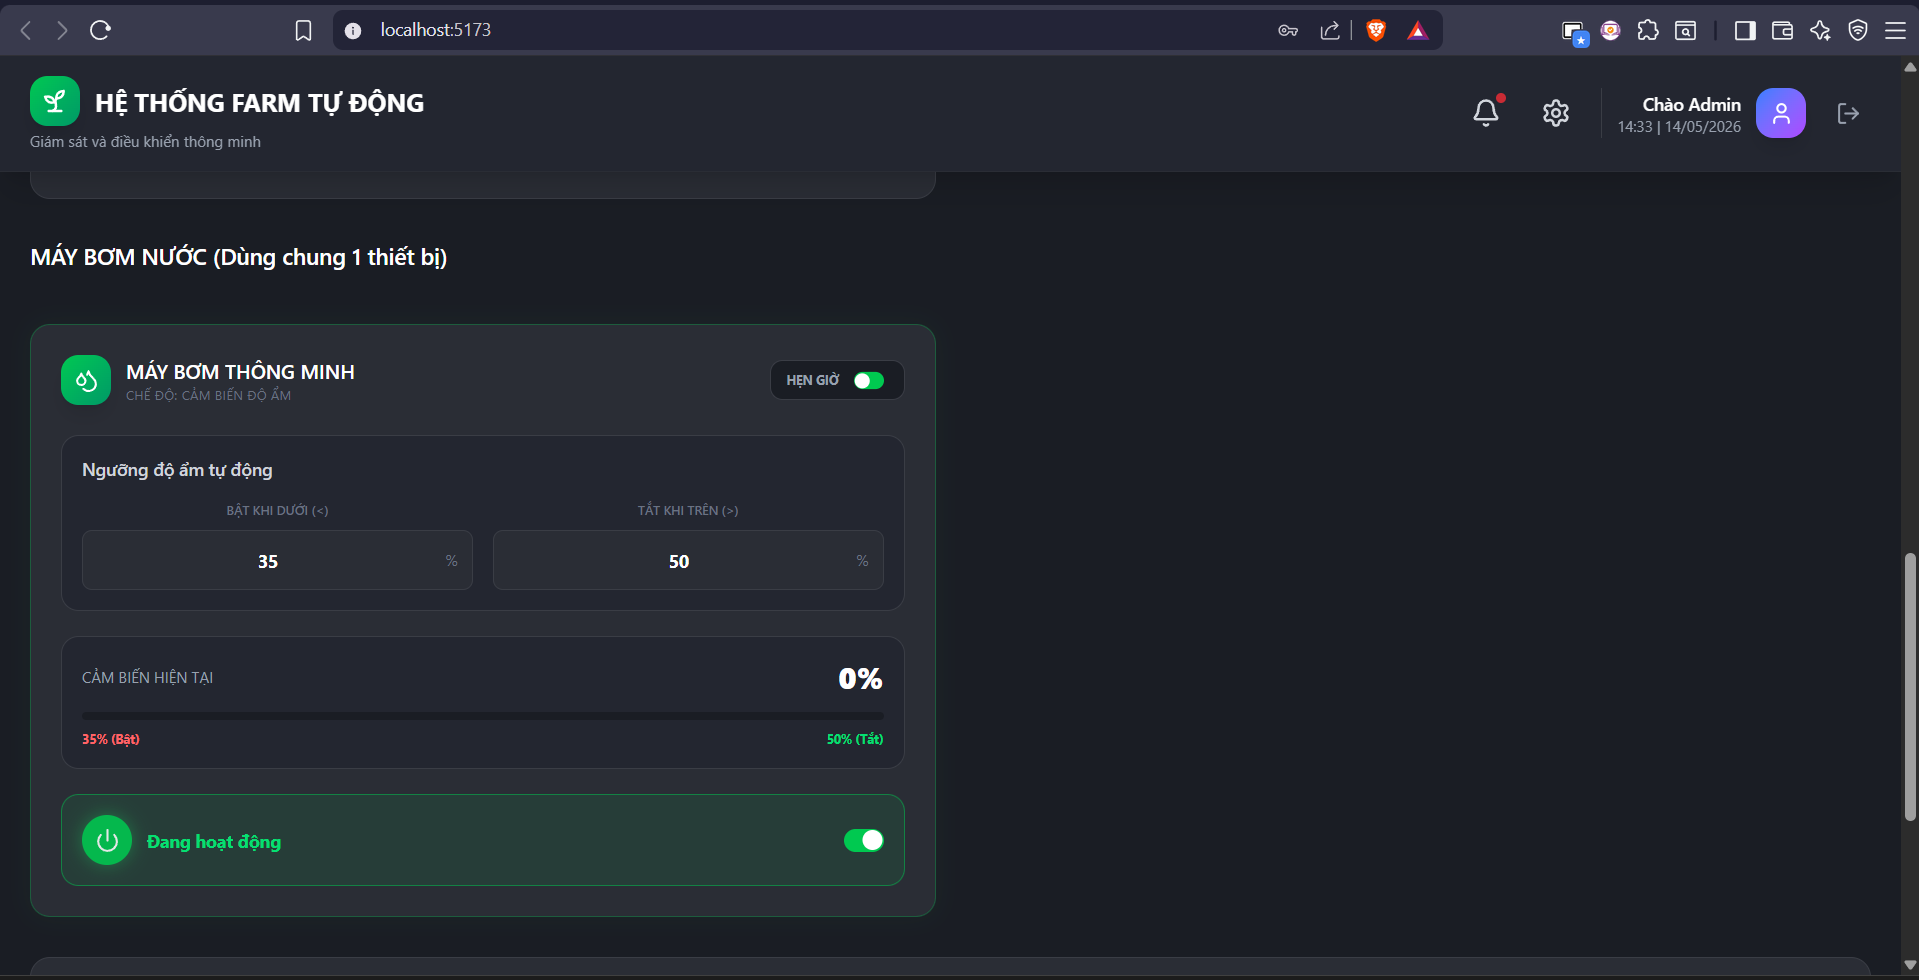
\includegraphics[width=\textwidth]{img/maybomdoam.png}
    \caption{Giao diện điều khiển máy bơm theo ngưỡng độ ẩm}
    \label{fig:interface2}
  \end{subfigure}
  
  \caption{Tổng hợp giao diện điều khiển máy bơm}
  \label{fig:overall_interface}
\end{figure}
Ở đây có thể điều khiển thiết bị máy bơm bằng 2 cách: 
\begin{itemize}
  \item Điều khiển thủ công: người dùng có thể bật/tắt máy bơm theo ý muốn.
  \item Điều khiển tự động: người dùng có thể cài đặt thời gian bật tắt hoặc các ngưỡng về độ ẩm đất, nếu độ ẩm đất thấp hơn ngưỡng đã cài đặt thì máy bơm sẽ tự động bật, nếu độ ẩm đất cao hơn ngưỡng đã cài đặt thì máy bơm sẽ tự động tắt.
\end{itemize}
\subsubsection{Điều khiển đèn LED}
\begin{figure}[H]
  \centering
  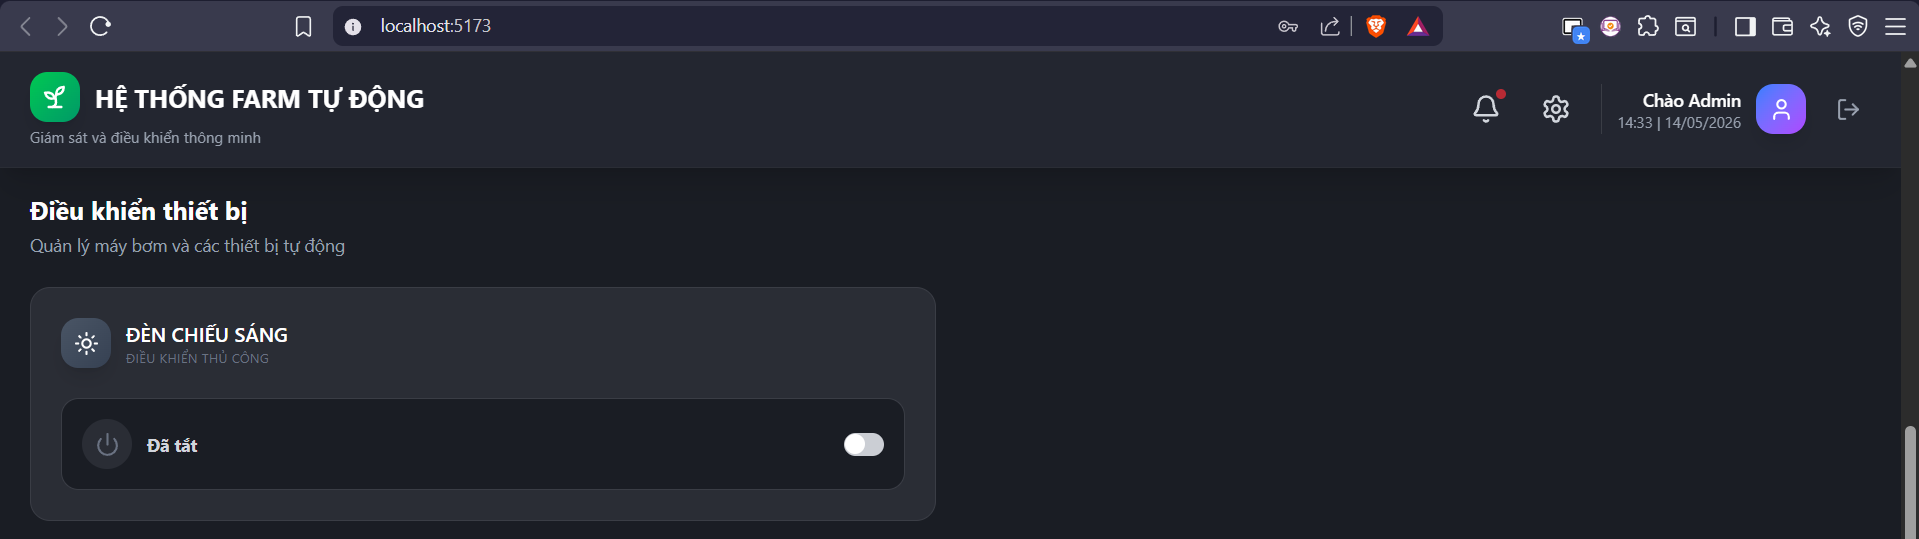
\includegraphics[width=0.8\textwidth]{img/dkden.png}
  \caption{Giao diện điều khiển đèn LED}
  \label{fig:interface}
\end{figure}
\subsection{Giao diện xem thông báo và nhật kí}
Người dùng có thể xem các thông báo về tình trạng thiết bị máy bơm bật/tắt, các cảnh báo về điều kiện thời tiết, và nhật kí hoạt động của hệ thống.

\begin{figure}[H]
  \centering
  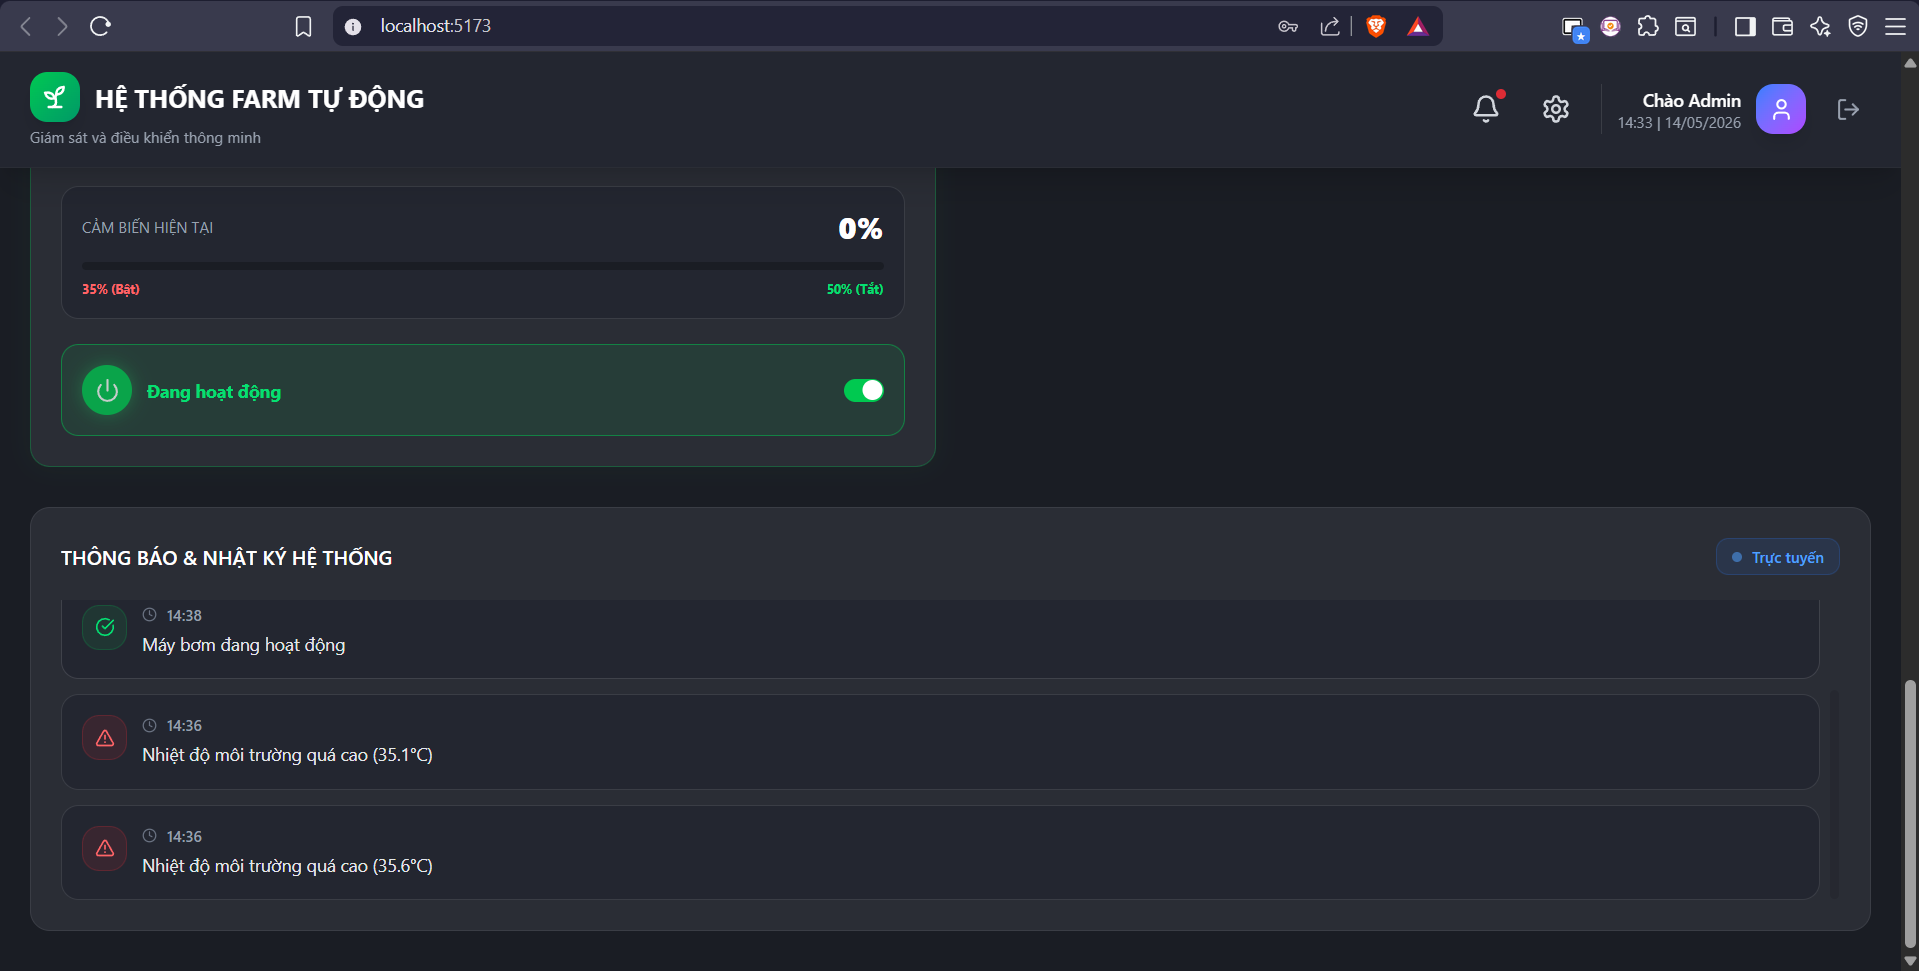
\includegraphics[width=0.8\textwidth]{img/thongbao.png}
  \caption{Giao diện xem thông báo và nhật kí}
  \label{fig:interface}
\end{figure}


\subsection{Giao diện xem lịch sử dữ liệu}
Người dùng có thể xem lịch sử dữ liệu cảm biến (nhiệt độ, độ ẩm không khí, ánh sáng) theo thời gian được lưu lại trên cơ sở dữ liệu. Dữ liệu được hiển thị dưới dạng biểu đồ để người dùng dễ dàng theo dõi và phân tích xu hướng của các thông số môi trường trong nông trại.
\begin{figure}[H]
  \centering
  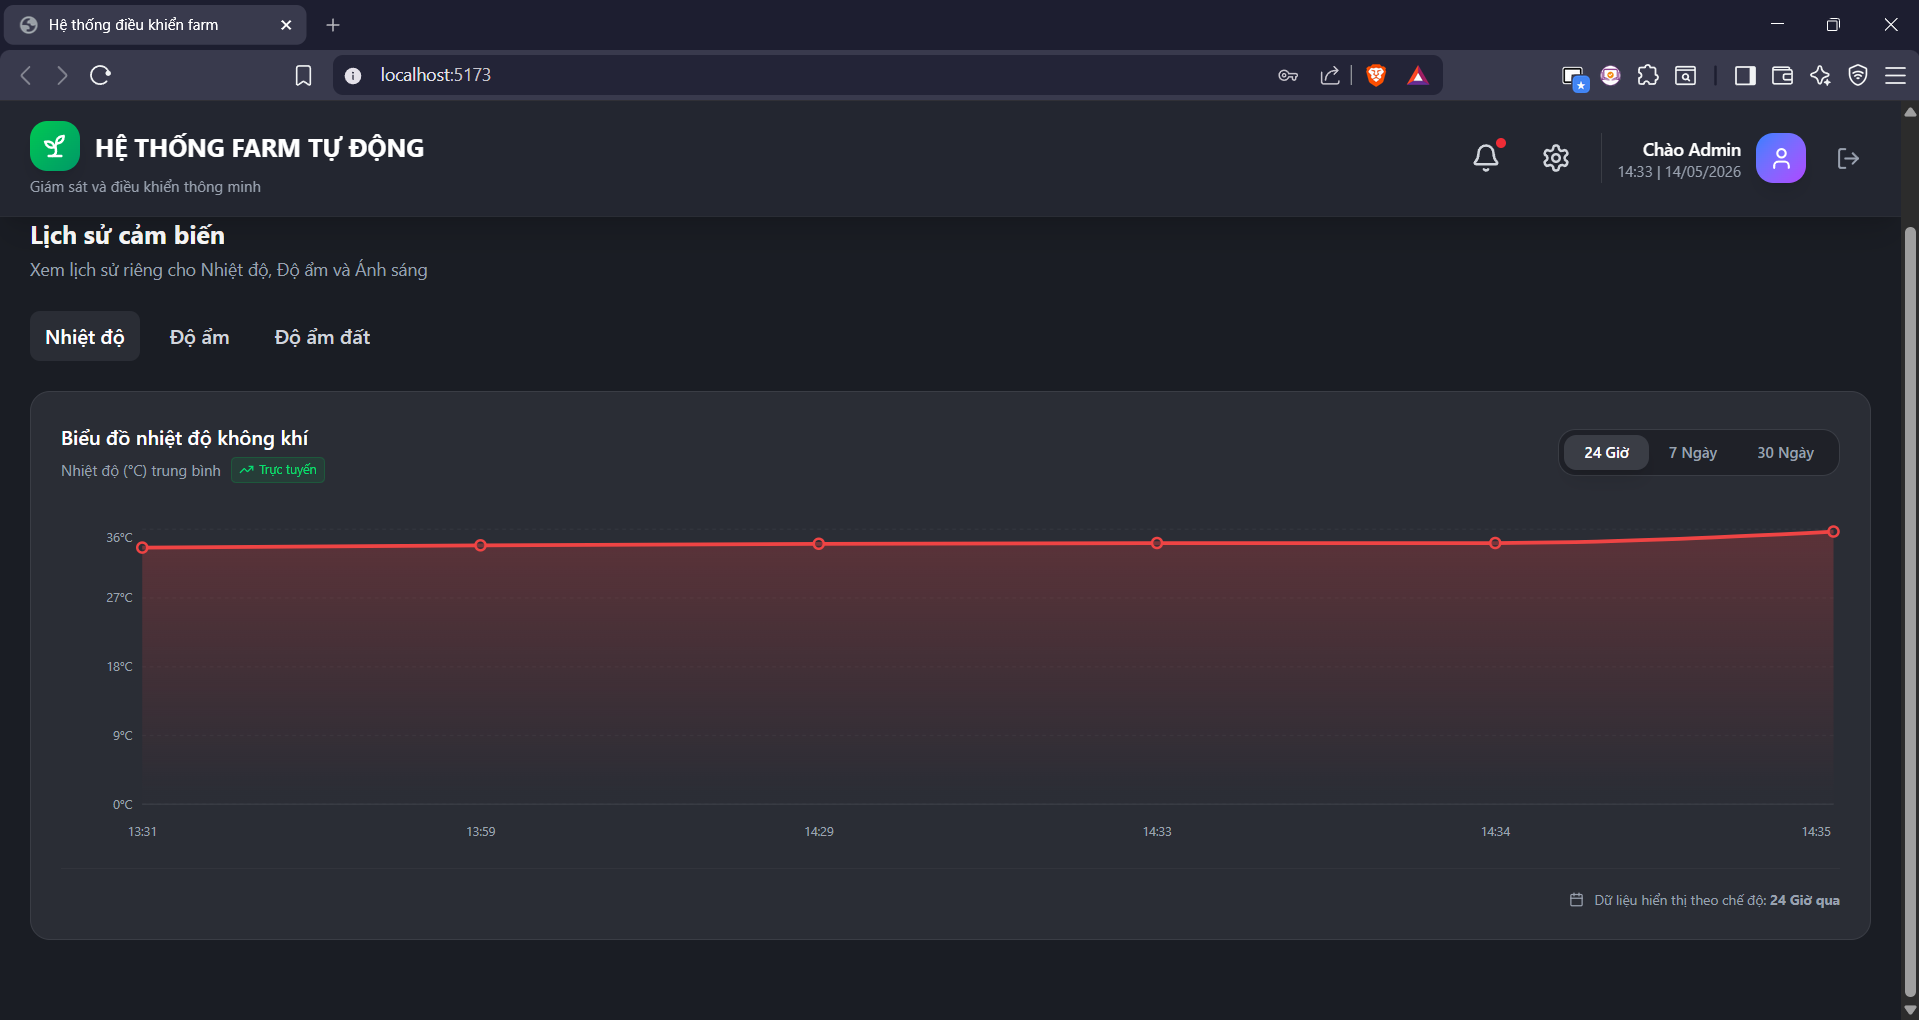
\includegraphics[width=0.6\textwidth]{img/lichsunhietdo.png}
  \caption{Giao diện xem lịch sử nhiệt độ}
  \label{fig:interface}
\end{figure}

\begin{figure}[H]
  \centering
  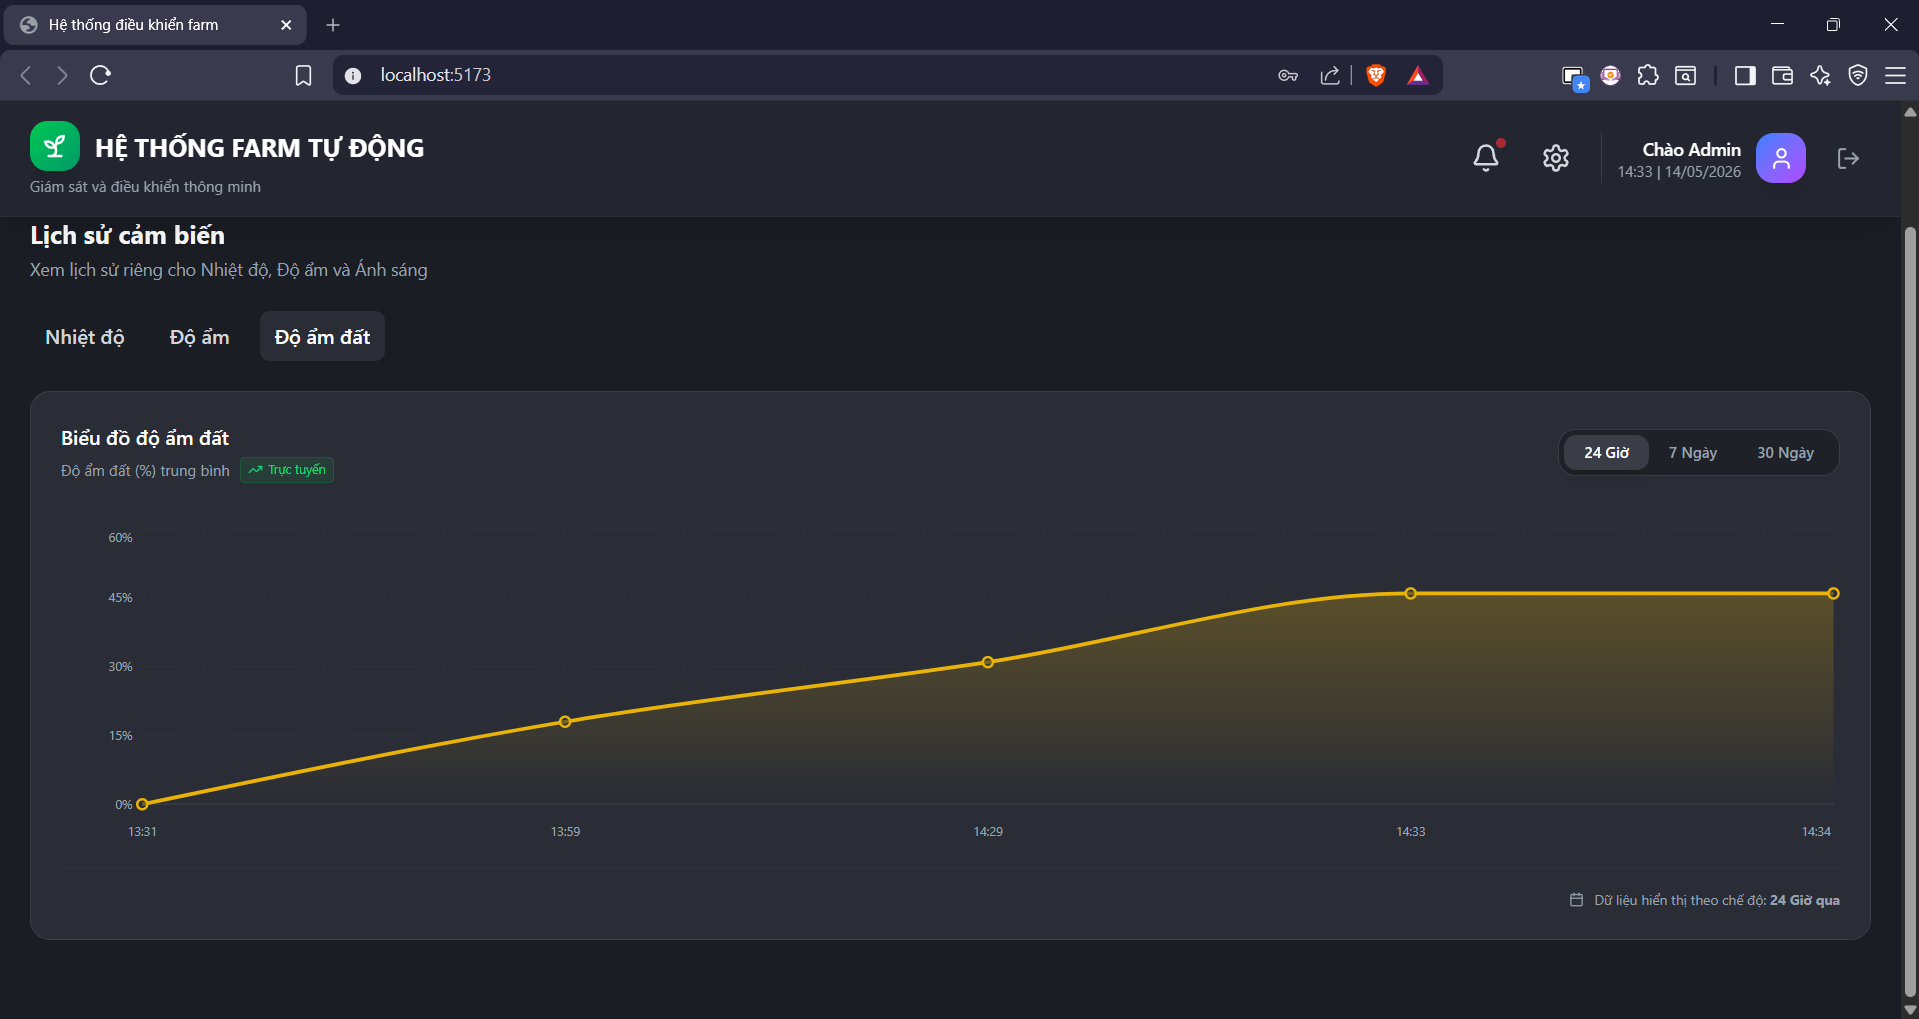
\includegraphics[width=0.6\textwidth]{img/lichsudoamdat.png}
  \caption{Giao diện xem lịch sử độ ẩm đất}
  \label{fig:interface}
\end{figure}

\begin{figure}[H]
  \centering
  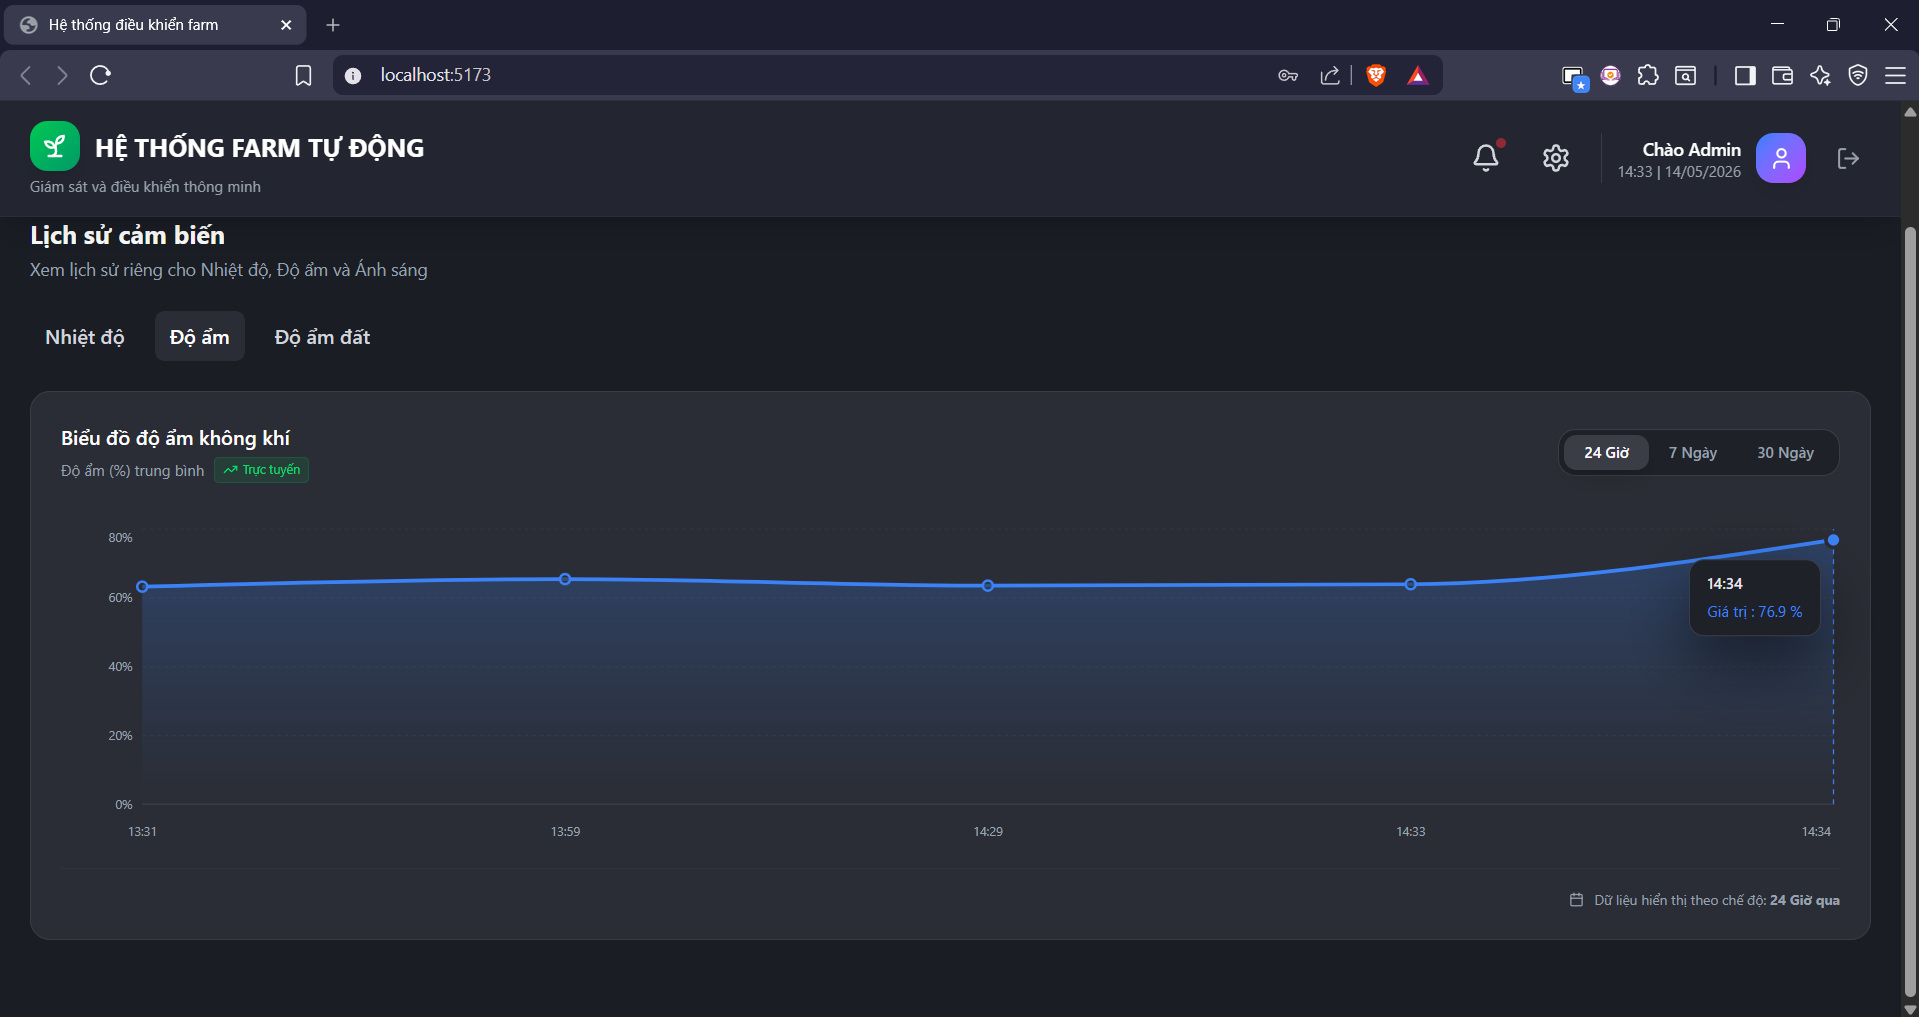
\includegraphics[width=0.6\textwidth]{img/lichsudoamkk.png}
  \caption{Giao diện xem lịch sử độ ẩm không khí}
  \label{fig:interface}
\end{figure}

\section{Triển khai kết nối thiết bị bằng app.ohsystem.vn và dashboard cơ bản trên Adafruit}
\subsection{Triển khai trên ohsystem}
\begin{figure}[H]
    \centering
    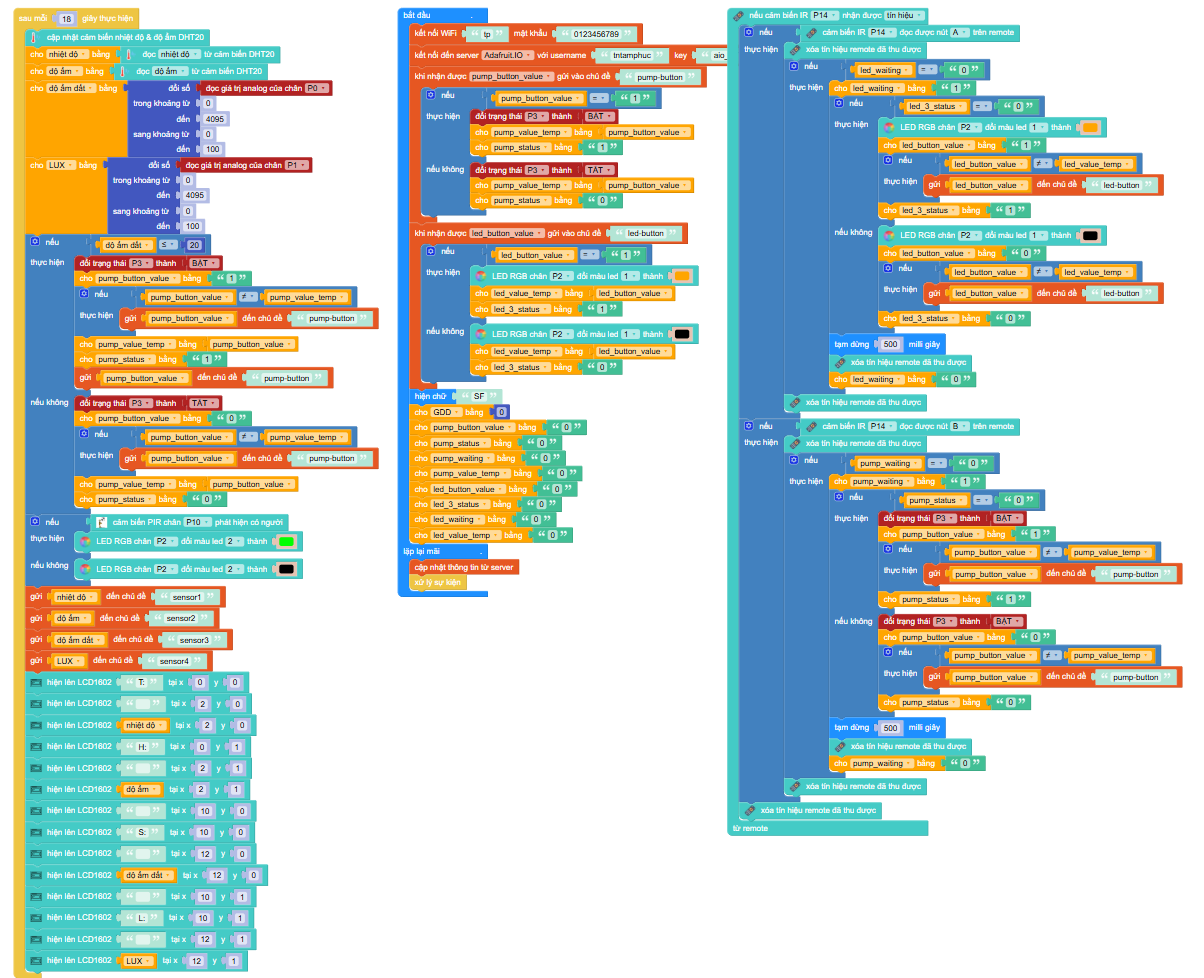
\includegraphics[width=0.8\textwidth]{img/ohsytem.png}
    \caption{Triển khai kết nối thiết bị trên ohsystem}
\end{figure}

\subsection{Dashboard cơ bản trên Adafruit}
\begin{figure}[H]
    \centering
    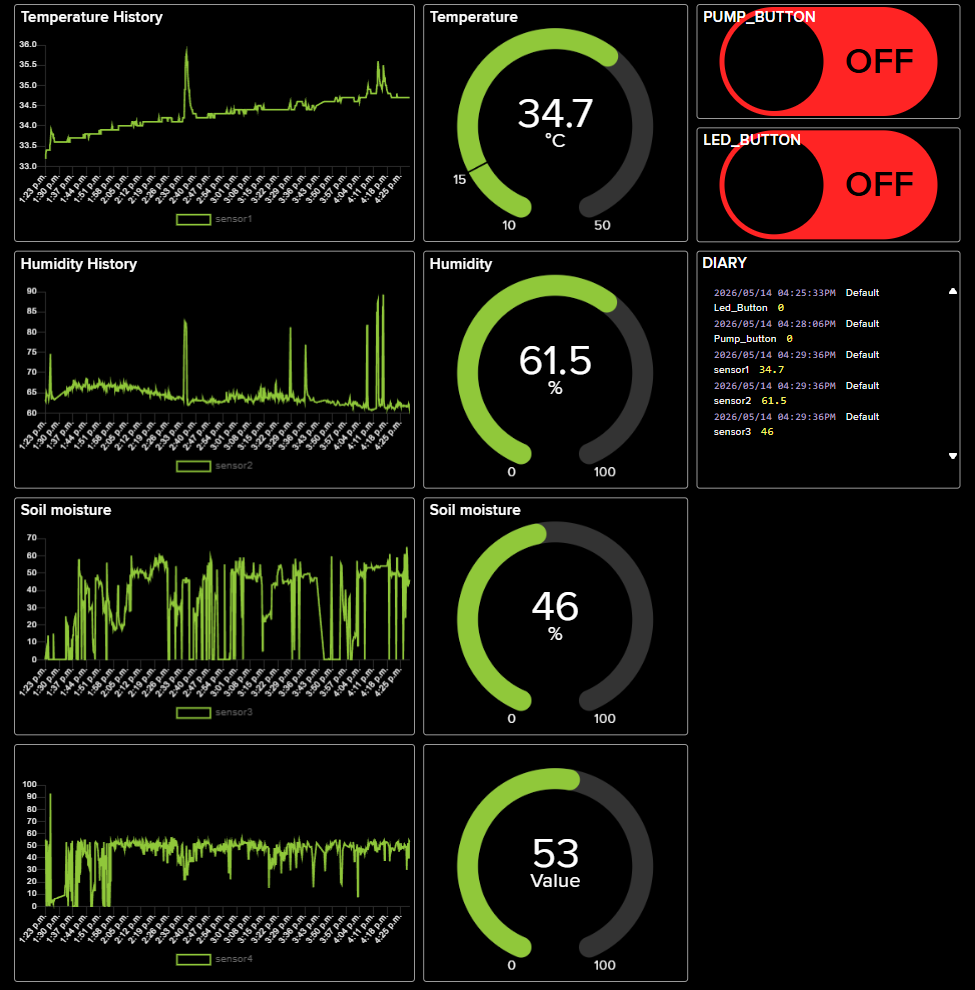
\includegraphics[width=0.8\textwidth]{img/adafruit.png}
    \caption{Dashboard cơ bản trên Adafruit}
\end{figure}
